\pdfcompresslevel9
\pdfdecimaldigits2
\pdfminorversion4

\documentclass[12pt,a4paper]{book}
\usepackage[bottom=2.5cm,top=3.5cm]{geometry}
%\usepackage{ngerman}
\usepackage[utf8]{inputenc}
\usepackage[T1]{fontenc}
\usepackage{graphicx}
\usepackage{colortbl}
\usepackage{ae}
\usepackage{amssymb}
\usepackage{amsmath}
\usepackage{amsthm}
\usepackage{multirow}
\usepackage{rotating}
\usepackage[margin=10pt,font=small,labelfont=bf]{caption}
\usepackage{listings}
\usepackage{microtype}

%\linespread{1.25}
\setlength{\parindent}{0pt}

\usepackage{fancyhdr}
\usepackage[
  	pdfstartview=FitH,   
  	pdffitwindow=true,
	pdftitle = "Models of Computation WiSe1011 UdS", % Sets the document information Title field
    pdfauthor = "Adrian Neumann", %Sets the document information Author field
  	colorlinks,
  	linkcolor=black,
  	anchorcolor=black,
  	citecolor=black,
  	urlcolor=black
]{hyperref}

\pagestyle{fancy}
\cfoot{\thepage}

\newsavebox{\footerlicence}
\sbox{\footerlicence}{
\includegraphics{./images/by-nc-sa}}

\rfoot{\usebox{\footerlicence}}
\fancyhead{}
\lfoot{Found a mistake? Write an e-mail!}

\definecolor{gruen}{rgb}{0.5,1,0.5}
\definecolor{rot}{rgb}{1,0.5,0.5}


\renewcommand{\footrulewidth}{0.4pt}
\renewcommand{\headrulewidth}{0pt}
\newcommand{\B}[0]{\mathbb{B}}
\newcommand{\N}[0]{\mathbb{N}}
\newcommand{\Z}[0]{\mathbb{Z}}
\newcommand{\Q}[0]{\mathbb{Q}}
\newcommand{\R}[0]{\mathbb{R}}
\newcommand{\C}[0]{\mathbb{C}}
\newcommand{\E}[0]{\mathbb{E}}
\newcommand{\im}[0]{\mathit{i}}
\newcommand{\kthings}[2]{{#1}_1,\ldots,{#1}_{#2}}
\newcommand{\nthings}[1]{\kthings{#1}{n}}
\newcommand{\norm}[1]{|\!|#1|\!|}
\newcommand{\rank}{\mbox{rank }}
\newcommand{\skal}[1]{\left\langle {#1} \right\langle}
\newcommand{\ok}{{\large \checkmark}}
\newcommand{\no}{{\large $\mathbb{\times}$}}
\newcommand{\nz}{\text{nz}}
\newcommand{\rup}[1]{\left\lceil #1 \right\rceil}
\renewcommand{\bar}{\overline}
\renewcommand{\arraystretch}{1.5}
\newcommand{\argmin}[1]{\underset{#1}{\operatorname{argmin}}}
\newcommand{\var}{\operatorname{var}}



\newcommand{\trans}[1]{{#1}^\text{\upshape \sffamily T}}
\newtheoremstyle{leplain} %name
    {2em} %above
    {2em} %below
    {} %body font
    {} %indent
    {\bfseries} %head font
    {:} %punctuation after head
    {0.5em} %space after head
    {} %head spec
\title{Models of Computation}
\author{Adrian Neumann \\ {\small \texttt{adrian\_neumann@gmx.de}}}


\date{}

\begin{document}
\frontmatter
\lstdefinelanguage{pseudocode}{
    morekeywords = {repeat, until, if, else, wait, send, receive, unless, while, for, return, break},
    sensitive = false,
    morecomment=[l]{//},
    morecomment=[s]{/*}{*/},
}
\lstset{language=pseudocode, basicstyle=\sffamily\small, commentstyle=\slshape\sffamily, keywordstyle=\upshape\bfseries, breaklines=true, mathescape=true, tabsize=2}


\theoremstyle{definition}
\newtheorem{Def}{Definition}[section]

\theoremstyle{leplain}
\newtheorem{ex}{Example}[section]
\newtheorem{pr}{Proof}[section]
\newtheorem{cor}{Corollary}[section]
\newtheorem{lem}{Lemma}[section]

\theoremstyle{theorem}
\newtheorem{thm}{Theorem}[section]



\maketitle
\thispagestyle{fancy}

\section*{Disclaimer}

Most likely this script is riddled with errors so take everything with an appropriate dose of salt. Send the author emails or patches if you find errors or have some clarifications. 

These notes are released under a Creative Commons Attribution--Noncommercial--Share-Alike licence. So you can do pretty much everything with them as long as you mention the original authors, don't sell your work and distribute it under an equivalent licence. Read the licence agreement for details. Although the licence does not request it the author would be happy if you noticed him should you decide to use this.

\section*{Thanks}
The following persons have contributed:

\begin{center}
\begin{tabular}{l|c}
Name & Corrections\\\hline
Aram Harutyunan & 11
Radu Curticapean & 20
\end{tabular}
\end{center}
\newpage

\mainmatter

\chapter{Distributed Computing}

\section{Introduction}

Many autonomous entities with their own hardware (memory, CPU) in a system that connects them through a network over which they can send messages to each other. The natural way to represent that is a graph. There are many models to describe different aspects of the system. They have to deal with the following issues:

\begin{enumerate}
\item Communication. Usually communication is very expensive, its cost dominates all other costs. Hence it is typically assumed that communication is the only cost that occurs.
\item Fault Tolerance. In large computer networks it's common that a few nodes fail during the computation. Robustness against this is desirable. Results should be reasonable even if single entities fail.
\item Locality. Networks change over time, communicating these changes to all nodes would be too costly. It's better to design algorithms that only rely on local information.
\item Synchronization. Individual entities can have different hardware and solve problems at different speeds. It's good if algorithms don't have to assume synchronous computation.
\item Symmetry breaking. Nodes have to be made distinguishable.
\end{enumerate}

\section{Vertex Coloring}

Given an undirected graph $G=(V,E)$ we want to find a colouring, i.e. an assignment of colours $c_v$ to the vertices $v\in V$, such that no two adjacent vertices have the same colour.

This is useful for symmetry breaking. For example cellphones that communicate with the same cell have to choose different frequencies.

We will assume that initially all nodes are equipped with a unique ID$\in [1,n]$. Typically each ID uses $O(\log n)$ bits. Obviously the IDs are a valid colouring. We want to try to use fewer colours, if possible the minimal number.

\begin{Def}[Chromatic Number] The chromatic number $\chi(X)$ of a graph is the minimal number of colours needed in any valid colouring of G.
\end{Def}

Computing the chromatic number is NP-complete. Hence we want to try to find some approximate solution.

A simple, sequential algorithm assigns colours greedily:

\begin{lstlisting}
Greedy(graph G)
while $\exists$ uncoloured vertex v
	colour v with min ([1,n] - colours(neighb(v)))
\end{lstlisting}

\begin{thm} The greedy algorithm stops after $n$ steps and produces a valid colouring and uses at most $\Delta(G)+1$ colours\footnote{$\Delta(G)$ is the maximal degree of the graph}.
\end{thm}

\begin{pr} It is clear that the algorithm stops in $n$ steps, since in each iteration the number of vertices decreases by one. 

Correctness is given by an inductive argument. During the execution the coloured subgraph is always valid, since we assign colours that don't occur in the neighbourhood.

Finally $\Delta(G)+1$ is an upper bound for the number of colours since there is always a free colour in the set $[1,\Delta(G)+1]$ 
\end{pr}

We want to construct a distributed algorithm that uses the same ideas to reduce the number of colours.

\begin{lstlisting}
First-Free(coloured G, vertex v)
	give v the smallest available colour
\end{lstlisting}

This algorithm can produce error if two adjacent vertices choose the colour at the same time under certain circumstances.

\begin{figure}
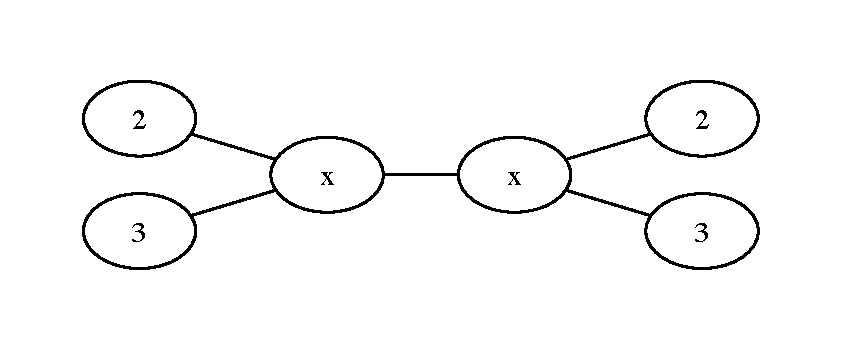
\includegraphics[width=0.5\linewidth]{./images/graph1}
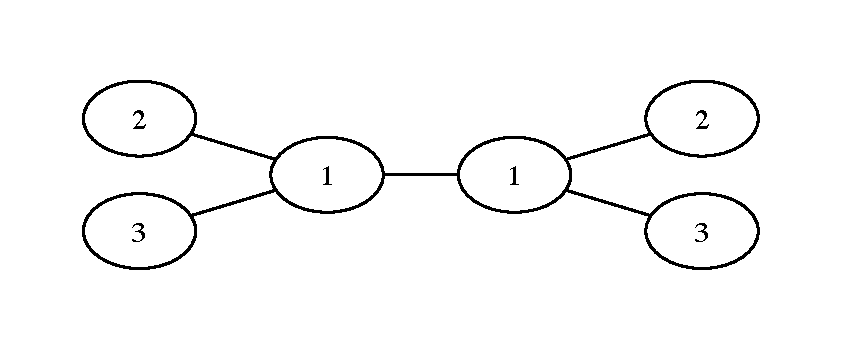
\includegraphics[width=0.5\linewidth]{./images/graph11}
\caption{If the nodes labelled with x have high IDs and choose simultaniously they produce an invalid colouring.}
%n1 2
%n2 x
%n3 3
%n4 10
%n5 2
%n6 3
%n1 -- n2
%n2 -- n3
%n2 -- n4
%n4 -- n5
%n4 -- n6
%
%n1 and n2 choose colours simultaniously, both get 1.
\end{figure}

It depends on the model how we can deal with this. Either we have the means for synchronisation, or we don't.

\begin{Def}[Synchronous Distributed Algorithm] During one unit of time an entity in a SDA can execute (in any order) the following things
\begin{itemize}
\item Perform local computations
\item Send messages
\item Receive messages
\end{itemize}

As long as they are of "reasonable" complexity
\end{Def}

In this model we can change the algorithm like this:

\begin{lstlisting}
Reduce
	send own ID to all neighbours
	receive IDs from all neighbours
	while $\exists$ uncolored vertex in the neighbourhood that has larger ID
		send "undecided" to all neighbours
		receive messages from neighbours
	colour thyself with First-Free
	send the colour to neighbours
\end{lstlisting}

\begin{thm} Reduce is correct, i.e. it produces a valid colouring after at most $n$ rounds. The number of colours used is upper bounded by $\Delta(G)+1$. 
\end{thm}

\begin{pr}
\end{pr}
\subsection{Colouring Trees}

In order to finde a faster algorithm we first look at a special case, trees. A tree is an acyclic connected graph. All trees are bipartite, and hence have chromatic number 2.

\begin{thm} $T$ is a tree implies $\chi(T)=2$ \end{thm}

\begin{pr} Let $v$ be a distinguished vertex, the root, in the tree. Colour $v$ red.  Colour every other vertex according to the distance from the root. If the distance is odd colour it blue, else red. Since there are no cycles in the graph, the coloring is valid.
\end{pr}

If we assume that the root knows that it's special we can construct the algorithm in figure \ref{alg:slow_tree_colour}

\begin{figure}[hbt]
\begin{lstlisting}
root: colour with red; send to all children
all except root: 
	wait for message
	if parent red
		colour blue
	else
		color red
	send colour to all children
\end{lstlisting}
\caption{Slow Tree Coloring}
\label{alg:slow_tree_colour}
\end{figure}


This algorithm isn't faster than the previous one, for degenerate trees. We also need to find a way to decide which node is the root. The latter problem is deferred to a later lecture.

Note that this algorithm doesn't need to operate in a synchronous environment. Every node waits for an event before it starts its computation. Event-driven algorithms can be implemented in asynchronous settings

\begin{Def}[Asynchronous DA] A asynchronous distributed algorithm has no access to a global clock and works event-driven.

Any sent message will arrive in finite time.
\end{Def}

There are different ways to assess the complexity of asynchronous algorithms (there are not bounds on the time a message takes). Typically we are interested in 

\begin{itemize}
\item Message Complexity: The number of messages sent
\item Time Complexity: Under the assumption that each message has delay 1, the time complexity is the length of the longest chain of interdependent messages.
\end{itemize}

\begin{thm} The asynchronous time complexity of algorithm \ref{alg:slow_tree_colour} is $\leq height(T)$ \end{thm}
\begin{pr} In the first round the root sends its colour to all neighbours. This costs one time unit. Argument follows from induction on the height\end{pr}

We now try to improve the algorithm to get a better runtime than $O(n)$. In fact we'll give an algorithm that is bounded by $O(\log^*n)$. We assume that all vertices know that the graph is a tree, a root is known and each node knows it's parent. How we find that information is again deferred to later

\begin{figure}[hbt]
\begin{lstlisting}
Let $c_v$ be ID(v)
repeat 
	send $c_v$ to all childrens
	if $v$ is the root then
		I=0
	else 
		let $c_p$ be the parent's colour
		I = smallest i s.t. bin$_i$($c_v$), bin$_i$($c_p$) differ
		$c_v$ = <bin(I),bin$_I$($c_v$)> //use $1+\log |c_v|$ bits  
		                                //even if I small
until |bin($c_v$)| does not change
\end{lstlisting}
\caption{6-colour}
\label{alg:6-colour}
\end{figure}

\begin{lem} Algorithm \ref{alg:6-colour} produces a valid colouring \end{lem}

\begin{pr} Since all IDs are different the colouring is valid in the first step. Now consider some iteration during the execution of the algorithm

Let $u$ be the parent of $w$. If $u$ finds $I_u$ and $w$ finds $I_w$ then the new colours are $c_u=<bin(I_u), bin_{I_u}(c_u)>, c_w<bin(I_w),b_{I_w}(c_w)>$. There are two cases

\begin{itemize}
\item $I_u\neq I_w$. Then the first part of the new colours differ. \ok
\item $I_u=I_w=I$. Then we have $b_I(c_u)\neq b_I(c_w)$, by the choice of $I$ \ok
\end{itemize}

So the colouring stays valid after each round.
\end{pr}

\begin{lem} Let $K_i$ be the number of bits in the representations of the colours in round $i$.

\begin{align*}
K_0 &= \left\lceil \log n\right\rceil\\
K_{i+1} &= 1+\left\lceil K_i\right\rceil
\end{align*}

\end{lem}

\begin{pr}
We have that $K_{i+1} < K_i$ as long as $K_i\geq 4$. If $K_i\in \{1,2,3\}$, we have $K_{i+1}=K_i$. Otherwise we can write $K_i=2^x\cdot y$, $x\in \N$, $y\in [1,2)$. Then we have

\[K_{i+1} = 1+\left\lceil \log(2^x\cdot y)\right\rceil = \begin{cases} 1+x & y=1\\ 2+x &y>1\end{cases}\]

So we have 

\[K_{i+1}<K_i \Leftrightarrow 2^x\cdot y > \begin{cases} 1+x & y=1\\ 2+x &y>1\end{cases}\]

check yourself that the exponential function on the left grows sufficiently fast for the claim to be true.
\end{pr}

\begin{thm} The final colouring uses at most 6 colours and stops after $O(\log^* n)$ rounds.\end{thm}

\begin{pr} Let $i$ be the final iteration. Since the algorithm stopped, we know $K_i=K_{i-1} \leq 3$. The colour is encoded as $<bin(I), bin_I(c)>$ since $I\leq 3$ we get only six possible colours.

For the running time we claim: $K_i\leq 2+ \left\lceil \log^{(i)} K_0 \right\rceil$. This can be proven by induction on $i$. 

$i=1$ \ok. $i\rightarrow i+1$:

\begin{align*}
K_{i+1}&= 1+\rup{\log K_i}\\
	&\leq 1+ \rup{\log(2+\rup{\log^{(i)}K_0})}\\
	&\leq 1+\rup{1+\log \rup{\log^{(i)} K_0}}\\
	&\leq 2+\rup{1+\log \rup{\log^{(i)} K_0}}\\
	&=\leq 2+\rup{1+\log \log^{(i)} K_0}\\
\end{align*}

If we choose $i=\log^*(K_0)$ we get $K_i\leq 4$ by definition of $\log^*$. Henc in round $\log^*(K_0)+2$ the algorithm will finish.
\end{pr}

Six colours isn't very satisfying for a bipartite graph, so we try to reduce the number of colours further.

\begin{figure}[hbt]
\begin{lstlisting}
root: choose a different colour
all others: take the old colour of parent
\end{lstlisting}
\caption{Shift-Down}
\label{alg:Shift-Down}
\end{figure}

Algorithm \ref{alg:Shift-Down} only takes one round.

\begin{lem} The colouring produced by algorithm \ref{alg:Shift-Down} is valid, if the intitial colouring is valid. Also, all siblings of a node have the same colour.\end{lem}

\begin{pr} Let $c'_u$ be the initial colours and $c_u$ be the new ones. Let $u_1\rightarrow u_2 \rightarrow u_3$ be a path in the tree. Then $c_{u_2}=c'_{u_1} \neq c_{u_3}=c'_{u_2}$. The root is also ok, since it chooses a fresh colour.\end{pr}

\begin{figure}[hbt]
\begin{lstlisting}
For $x\in \{3,4,5\}$
	Shift-Down
	All vertices coloured with $x$ call First-Free
\end{lstlisting}
\caption{6-to-3}
\label{alg:6-to-3}
\end{figure}

\begin{lem} The colouring produced by \ref{alg:6-to-3} is valid and contains $\leq 3$ colours.\end{lem}

\begin{pr} After the shift down, the neighbourhood of a vertex labelled with $x$ contains only two colours. The colour of the parent and the colours of the children. It can also not happen that two adjacent vertices call First-Free simultaniously, since then they would have had the same colour to begin with.\end{pr}

Finding a colouring with just 2 colours is not possible as fast.

\subsection{Lower Bounds}
\subsection{Lower Bounds}

We're now going to prove that \ref{alg:6-colour} is optimal. Recall that we have the following assumptions:

\begin{itemize}
\item We're working in a synchornous model
\item We have an initial colouring
\end{itemize}

\begin{thm}\label{thm:ring_color_lowerbound} Any deterministic algorithm colouring any\footnote{the only thing that differs between the rings is the initial colouring. We basically claim there exists an initial colouring that produces that runtime.} ring with n nodes with at most three colours needs $\Omega(\log^* n)$ rounds.
\end{thm}

Consider a node $v$. After $t$ rounds it can discover information, i.e. the topology and the IDs, about a $t$-neighbourhood around it.

Assume the vertices can distinguish between clockwise and counterclockwise neighbours, s.t. we can impose some ordering on them (this can only speed up the algorithm, so the assumption is ok for proving lower bounds).

Define

\[W_{s,n} = \{(x_1,x_2,\ldots,x_s) | 1 \leq x_i\leq n, x_i\neq x_j\}\]

Essentially after $t$ rounds, each vertex sees an element from $W_{2t+1,n}$. So any distributed algorithm colouring any right with $\leq 3$ colours calculates a function

\[A:W_{2t+1,n} \longrightarrow \{1,2,3\}\]

in $t$ rounds. We will now show that this function doesn't exist if $t$ is not in $\Omega(\log^*n)$.

Define a graph as follows:

\[G_{s,n} = (W_{s,n},E_{s,n})\]

where there is an edge in between two elements of $W_{s,n}$ in $E_{s,n}$ if they overlap in all but the first and the last position, i.e. edges have the form $\{(x_1,x_2,\ldots,x_s),(x_2,x_3,\ldots,x_{s+1})\}$. So we have edges between neighbourhoods that correspond to neighbouring vertices in some ring.

\begin{figure}[hbt]
\begin{center}
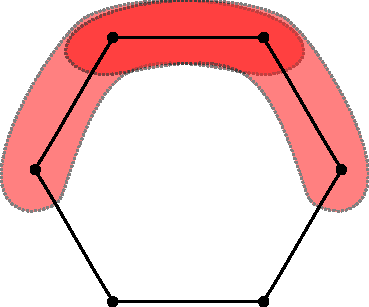
\includegraphics{./images/ring.pdf}
\end{center}
\caption{Overlapping 1-neighbourhoods on a ring}
\end{figure}

\begin{lem} The function $A$ is a valid colouring for the graph $G_{2t+1,n}$.\end{lem}

\begin{pr} Let $\{v,v'\}\in E_{2t+1,n}$ be an edge as above. Assume for the sake of contradiction that $A$ does not produce a valid colouring, i.e. $A(v)=A(v')$. We now construct a ring that is a valid input for the algorithm.

Consider the ring 

\[x_1\rightarrow \ldots \rightarrow x_{t+1} \rightarrow x_{t+2} \rightarrow \ldots \rightarrow x_{2t+1} \rightarrow x_{2t+2} \rightarrow \ldots \rightarrow x_1\] 

%picture ring with vertices x_1... x_t+1 x_t+2 ... x_2t+1,x_2t+2

Since the algorithm produces a valid colouring it colours $x_{t+1}$ and $x_{t+2}$ with different colours. But then the function must be $A(v)\neq A(v')$.
\end{pr}

It follows that $\chi(G_{2t+1,n})\leq 3$. We now show that the chromatic number is actually larger, if $t$ is too small.

\begin{Def} For a graph $\vec G$, the line graph $L(\vec D)$ is  the graph with the same vertex set as $\vec D$ and $(e,e')$ is an edge if e ends where e' starts. 

\begin{figure}[hbt]
\begin{center}
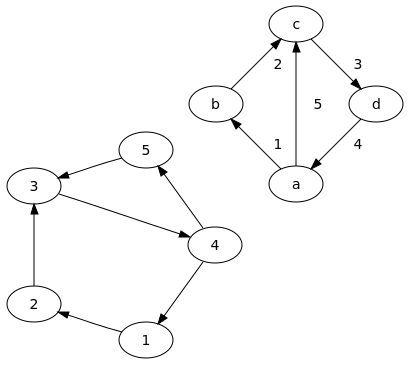
\includegraphics[width=0.8\linewidth]{./images/linegraph_ex}
\end{center}
\caption{A graph and its linegraph}
\end{figure}
\end{Def}

\begin{lem} $\chi(G_{2t+1,n}) \geq \log^{(2t)} n$\end{lem}

\begin{pr} Define a new, directed graph $\vec G_{s,n} = (\vec W_{s,n}, \vec E_{s,n})$ that is build from a subset of the originial graph

\[\vec W_{s,n} = \{(x_1,x_2,\ldots,x_s) | 1\leq x_1\leq \ldots \leq x_s \leq n\}\]
\[\vec E_{s,n} = \{(\underbrace{(x_1,\ldots,x_s)}_{v},\underbrace{(x_2,\ldots,x_{s+1})}_{v'})| v,v'\in \vec W_{s,n} \wedge x_{s+1} > x_s\}\]

Since both the edge and the nodeset of $\vec G$ is a subset of $G$, we immediately have $\chi(\vec G)\leq \chi(G)$. By introducing the new graph we gained the ability to recursively characterize $\vec G_{s,n}$.

\begin{enumerate}
\item $\vec G_{1,n}$ is the complete graph ($i\rightarrow i'$, if $i'>i$). This follows from the definition.
\item $\vec G_{s+1,n} = L(\vec G_{s,n})$

Take $s=3$ as example, see figure \ref{fig:g3_l3}.

\begin{figure}[hbt]
\begin{center}
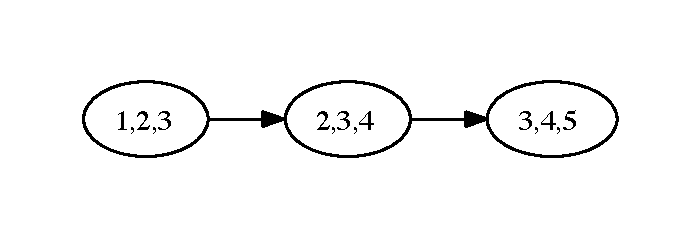
\includegraphics[width=0.58\linewidth]{./images/g3_extr} 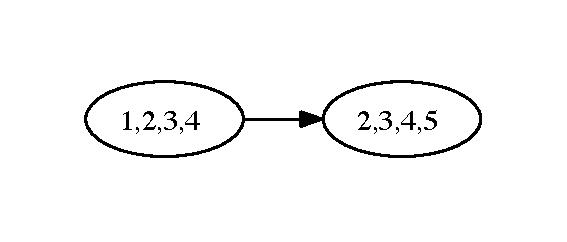
\includegraphics[width=0.4\linewidth]{./images/L(G3)}
\end{center}
\caption{A part of $\vec G_{3,n}$ and the corresponding part of $L(\vec G_{3,n})$}
\label{fig:g3_l3}
\end{figure}

We can identify the edges with elements from $\vec G_4$. And if we don't include an edge in the line graph, we also don't see it in $G_4$.

This also works in the general case: Every time we see an edge in $G_{s,n}$ we map the edge to the union of its endpoints, i.e. a node in $G_{s+1,n}$. If two edges are adjacent s.t. they are a new edge in the line graph, then the union is such that the edge is also in $G_{s+1,n}$
\end{enumerate}
\end{pr}

\begin{lem} $\chi(L(\vec D)) \geq \log \chi(\vec D)$ \end{lem}

\begin{pr} Let $k=\chi(L(\vec D))$ and $\phi$ be a k-colouring. $\phi$ is a colouring of the edges of $\vec D$, since it is a colouring of the line graph.

\begin{center}
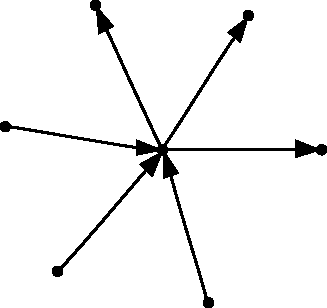
\includegraphics{./images/edge_coloring_line_graph}
\end{center}

For all incoming edges to a, all outgoing edges have a different colour in $\phi$, otherwise it wouldn't be a valid colouring for the line graph.

We construct a colouring $\hat \phi$ of $\vec D$ that uses at most exponentially more colours. 

\[\hat \phi(v) = (b_1,\ldots,x_k)\qquad b_i= \begin{cases} 1 & \exists \text{incoming edge with colour } i\\0 & \text{otherwise}\end{cases}\]

$\hat \phi$ is a valid colouring.

\begin{center}
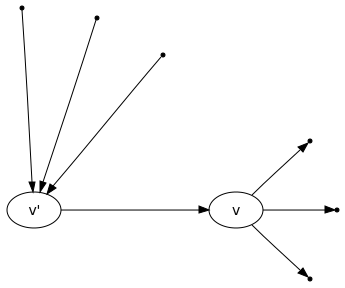
\includegraphics{./images/coloring_from_edges}
\end{center}

Suppose $b_i(v)=1$, then $b_i(v')=0$ otherwise we wouldn't have a valid edge colouring. Since we have $k$ bits available, we can use at most $2^k$ colours in $\hat \phi$.

\end{pr}

\begin{pr}[Theorem \ref{thm:ring_colour_lowerbound}] We need $t=\Omega(\log^* n)$ s.t. $\log^{(2t)} n$ is $\leq 3$.\end{pr}

\paragraph{Remark.}

\begin{itemize} 
\item$G_{s,n}$ doesn't have the nice recursive property. See the example in figure \ref{fig:g_3_counterex}

\begin{figure}[hbt]
\begin{center}
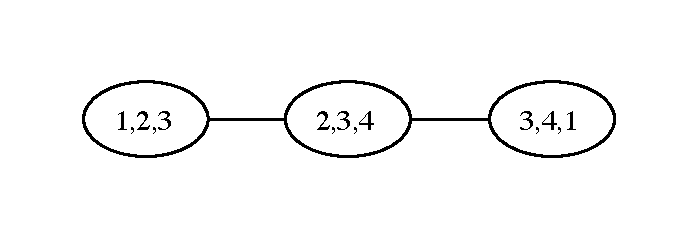
\includegraphics{./images/g_3_counterex}
\end{center}
\caption{The corresponding edge in the line graph $1,2,3,4 \rightarrow 2,3,4,1$ doesn't exist in $G_{4,n}$}
\end{figure}

%1,2,3 -- 2,3,4 -- 3,4,1
%
%a [label ="1,2,3"]
%b [label ="2,3,4"]
%c [label ="3,4,1"]
%
%a -- b -- c
%
%a [label ="1,2,3,4"]
%b [label ="2,3,4,1"]
%a -- b //does not exist
%1,2,3,4 -/- 2,3,4,1
\item The theorem \ref{thm:ring_colour_lowerbound} can be generalised to other graphs too.
\end{itemize}

\section{MIS --- Maximal Independent Set}

\begin{Def} Given an undirected graph $G=(V,E)$ an independent set $U\subseteq V$ is a subset s.t no two vertices in it are connected by an edge:

\[\forall u,v \in U \{u,v\}\not \in E\]

$U$ is \emph{maximal}, if no vertex can be added s.t. this property is preserved. Note the difference to a \emph{maximum} independent set: $U$ is \emph{maximum} if its cardinality is maximal among all independent sets.
\end{Def}

Note that the maximum set anddn a maximal set can be very different 

%picture 
\begin{figure}[hbt]
\begin{center}
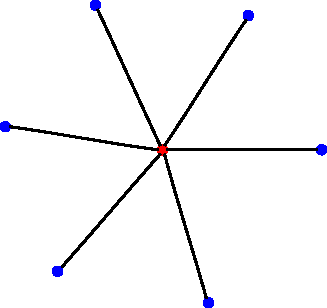
\includegraphics{./images/mis}
\end{center}
\caption{Red node is a maximal independent set, blue are a maximum independent set}
\end{figure}


Finding a maximum independent set is NP-complete, it is even inapproximable by a factor of $\approx \sqrt{n}$ unless P=NP. However maximal independent sets can be computed greedily. We want  to find a distributed algorithm for this problem.

There is a relation between colouring and MIS. Each color class in a coloured graph is an independent set, since there musn't be edges between nodes of the same colour. However it may not be maximal, but we can construct one in a distributed fashion by parallely adding vertices of other colours greedily.

\begin{thm} Given a synchronous distributed algorithm that colours a graph in $R$ rounds with $C$ colours, then we can find a MIS in time $O(R+C)$\qed\end{thm}

\begin{cor} There is a $O(\log^* n)$ algorithm for trees and bounded degree graphs\end{cor}

\subsection{A randomized algorithm}

Here we don't have to assume an initial colouring. Algorithm \ref{alg:fast_mis} runs in phases.

\begin{figure}
\begin{lstlisting}
repeat
	$c$ =  random [0,1] uniformly 
	send $c$ to all neighbour
	
	if $c_v< c_w$ for all $w\in adj(v)$ 
		enter MIS

until $v$ or $w\in adj(v)$ entered
\end{lstlisting}
\caption{Fast-MIS}
\label{alg:fast_mis}
\end{figure}

The algorithm terminates with probability 1, since with probability 1 there is a global smallest random choice, so at least one vertex stops in each round. It also produces a MIS, because as long as a vertex can enter, the algorithm won't stop.


We now want to show that this algorithm takes logarithmically many steps in expectation. We will look at the edges of the graph. We remove edges if they are incident to vertices that stop. We'll show that in expectation half the edges are removed in every round. 

Let $G_i=(V_i,E_i)$ be the graph at the beginning of the $i$th round. Obviously this is a random graph, as it results from a random process. Let $X_i$ be the random variable indicating the number of removed edges in phase $i$.

\begin{lem} \label{lem:at_least_half}$\E(X_i |G_i = G) \geq |E(G)|/2$ \end{lem}

\begin{pr} Define an event
\[E_{v\rightarrow v'} \forall w\in adj(v): c_v<c_w \wedge \forall w\in adj(v') \backslash {v} : c_v < c_w\]
to be the event that the edge ${v,v'}$ is removed because $v$ entered the maximal independent set and $v$ had the smallest random value of all neighbours of $v'$.

\begin{align*}
P(E_{v\rightarrow v'}) &= \frac{1}{| adj(v) \cup adj(v') |}\\
	&\geq \frac{1}{deg(v) + deg(v')}	
\end{align*}

Define a random variable 

\[Y_{v\rightarrow v'} = \begin{cases} \deg(v') & E_{v\rightarrow v'} \text{ occured} \\ 0 & \text{othw.}\end{cases}\]

that counts the edges that are incident to $v'$ and let $Y=\sum_{v,v'} Y_{v\rightarrow v'}$. By linearity of expectation we have

\begin{align*}
\E(Y) &= \sum_{v,v'} \E(Y_{v\rightarrow v'}) + \E(Y_{v'\rightarrow v}) \\
	&\geq \sum_{v,v'} \frac{d(v')}{d(v)+d(v')} + \frac{d(v)}{d(v')+d(v)}\\
	&= |E(G)|
\end{align*}

Let us now consider the relationship between $Y$ and $X_i$. Consider an edge $e={v,v'}$ as in figure \ref{fig:at_least_half} that is removed. $e$ gets counted in $Y$ if $E_{x\rightarrow v'}$ or if $E_{y\rightarrow v}$ happened. So each deleted edge gets counted up to two times. It can not happen that for example $E_{x'->v'}$ happens simultaneously with $E_{x\rightarrow v'}$, because we requested $x$ to be the minimal random value among all neighbours. Hence $X_i \geq Y/2$.

\begin{figure}
\begin{center}
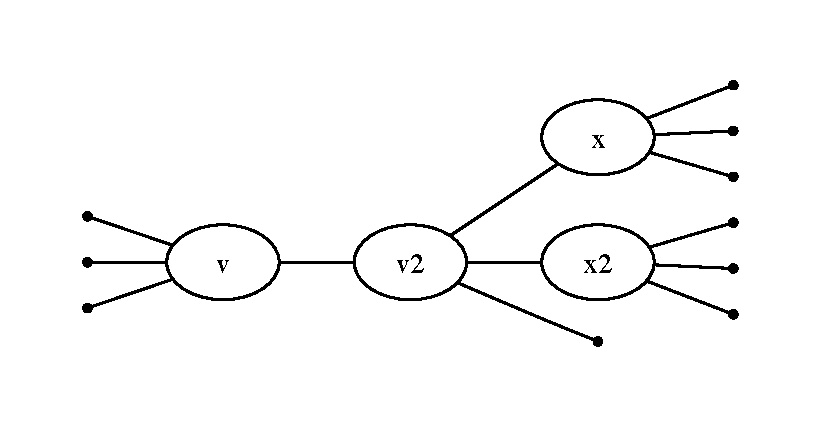
\includegraphics{./images/randomized_matching_delete_edge}
\end{center}
\caption{What edges can be deleted in one round?}
\label{fig:at_least_half}
\end{figure}
\end{pr}

Lemma \ref{lem:at_least_half} alone is not sufficient to prove the logarithmic running time, as the individual stages during the run of the algorithm are not independent\footnote{I think}. We need some more information before we can conclude the bounds on the running time.

\begin{lem} For all $i\geq 1$
\[P(|E_i| \geq 1) \leq |E_1| \cdot 2^{-i+1}\]
\end{lem}

\begin{pr} By Markov's inequality $P(|E_i| \geq 1) \leq \E(|E_i|)$. We want to show that $|E_i|\leq |E_1|\cdot 2^{-i+1}$.

We apply the law of total expectation\footnote{I think that's what it's called} and the previous lemma:

\begin{align*}
\E(|E_i|) &= \sum_{G\subseteq G_1} P(G_{i-1} =G) \cdot \E(|E_i| | G_{i-1}=G)\\
	&=\sum_{G\subseteq G_1}  P(G_{i-1} =G) \cdot \E(|E_{i-1}| -X_{i-1} | G_{i-1}=G)\\
	&=\sum_{G\subseteq G_1}  P(G_{i-1} =G) \cdot (\E(|E_{i-1}| | G_{i-1}=G) - \E( -X_{i-1} | G_{i-1}=G))\\
	&=\sum_{G\subseteq G_1}  P(G_{i-1} =G) \cdot (|E(G)| - \E(X_{i-1} | G_{i-1}=G))\\
	&\stackrel{\text{lem. \ref{lem:at_least_half}}}{=} \sum_{G\subseteq G-1}  P(G_{i-1} =G) \cdot (|E(G)| - \frac{|E(G)|}{2})\\
	&=\frac 12 \sum_{G\subseteq G-1}  P(G_{i-1} =G) \cdot |E(G)|\\
	&=\frac 12 \E(|E_{i-1}|)\\
\end{align*}

By induction we get the bound claimed in the lemma.
\end{pr}

\begin{lem} Let T be the number of rounds until Fast-MIS terminates. Then $\E(T) \leq 2\log n+O(1)$\end{lem}

\begin{pr} We have

\begin{align*}
\E(T) &= \sum_{i\geq 1} i P(T=i) \\
	&= \sum_{i\geq 1} P(T\geq i)\\
	&\leq C + \sum_{i> C} P(T\geq i)\\
\intertext{Note that $P\geq i$ implies $|E_i|\geq 1$, otherwise the algorithm would have stopped.}
	&\leq C+ \sum_{i> C} P(|E_i|\geq 1)\\
	&\leq C+ \sum_{i>C} |E_1|\cdot 2^{-i+1}\\
	&\leq C+ n^2 \cdot \sum_{i>C} 2^{-i}\\
	&\leq C+ n^2 \cdot 2\cdot 2^{-C}\\
\end{align*}

Choose $C$ to be $2\log n$ to get the result.
\end{pr}

\paragraph{Remark.} The algorithm may be fast in expectation, but that doesn't guarantee an acceptable running time with high probability. We would like to have a good running time with probability at least $1-n^{-c}$.

\begin{thm} $P(T> c\log n) = O(n^{2-c})$\end{thm}
\begin{pr} $T>i$ implies $E_i\geq 1$, so $P(T > i) \leq |E_1| \cdot 2^{-c\log n} = n^{2-c}$.\end{pr}

\paragraph{Remark.} \begin{enumerate}
\item We don't need to draw real numbers. It is sufficient to communicate $O(\log n)$ bits (exercise). 
\item It's an open problem to beat $O(\log n)$ randomized rounds. There is no known deterministic algorithm that has logarithmic running time.
\end{enumerate}

\subsection{Applications}

\subsubsection{General Graph Colouring}

We already know how to colour graphs of bounded degree in $O(\log^* n)$. We can use algorithm \ref{alg:fast_mis} to colour general graphs in logarithmic time. We construct an auxiliary graph $G^* = (V^*, E^*)$ out of $G$ by doing the following steps

\begin{enumerate}
\item For every $v\in V$ make $d(v)+1$ clones $C_v = \{v_0,v_1,\ldots v_{d(v)}\}$. $V^*$ is the set of all clones.
\item $C_v$ forms a clique in $G^*$
\item If $\{u,v\} \in E$ then $\{u_i,v_i\} \in E^*$ for $0\leq i \leq \min \{d(u),d(v)\}$, i.e. connect the cliques as in figure \ref{fig:colour_via_matching}

\begin{figure}
\begin{center}
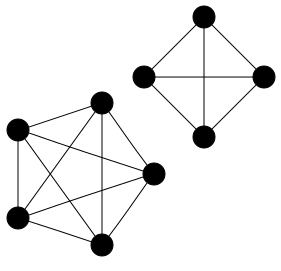
\includegraphics[scale=0.7]{./images/colour_via_matching}
%\begin{verbatim}
%graph G {
%
%	subgraph cluster2 {
%		label = "A"
%		a -- b
%		a -- c
%		a -- d
%		a -- e
%		b -- c
%		b -- d
%		b -- e
%		c -- d
%		c -- e
%		d -- e
%		
%	}
%	
%	subgraph cluster1 {
%	  label = "B"
%		f -- g
%		f -- h
%		f -- i
%		g -- h
%		g -- i
%		h -- i
%	}
%	
%	a -- f
%	b -- g
%	c -- h
%	d -- i
%}
%\end{verbatim}
\end{center}
\caption{Connecting the cliques}
\label{fig:colour_via_matching}
\end{figure}
\end{enumerate}

\begin{figure}[hbt]
\begin{lstlisting}
simulate Fast-Mis($G^*$) //only local information needed
if $v_i\in $ MIS, then
	$c_v=i$ 
\end{lstlisting}
\caption{An algorithm for general graph colouring}
\label{alg:general_colouring}
\end{figure}

\begin{thm} Algorithm \ref{alg:general_colouring} finds a valid colouring with $\leq \Delta+1$ colours in expected time $O(\log n)$.\end{thm}

\begin{pr} Observations:

\begin{enumerate}
\item Since the clones of a node are in a clique, at most one of them can be in the MIS
\item Let $v\in V$ be any vertex and let $w_1,\ldots,w_d$ be its neighbours in $G$

%picture
Since in the clique are $d+1$ vertices, but it only has $d$ edges to neigbouring cliques, one vertex must be free to join the MIS.

\end{enumerate}

So we get a colouring. We have to show that it's valid, i.e. the indices chosen into the MIS are not equal for neighbouring cliques. But this is obvious, since we have $\{u_i,v_i\}$ edges between cliques.

Since copying the nodes only makes the graph polynomially larger, the logarithmic running time is preserved.
\end{pr}

\end{document}
